\documentclass{beamer}

\usefonttheme{professionalfonts} % using non standard fonts for beamer
\usefonttheme{serif} % default family is serif

\usepackage{enumitem}
\setitemize{label=\usebeamerfont*{itemize item}%
  \usebeamercolor[fg]{itemize item}
  \usebeamertemplate{itemize item}}

\usepackage{hyperref}
%\usepackage{minted}
\usepackage{animate}
\usepackage{graphicx}
\def\Put(#1,#2)#3{\leavevmode\makebox(0,0){\put(#1,#2){#3}}}
\usepackage{colortbl}
\usepackage{tikz}
\usepackage{amssymb}
\usepackage{enumerate}
\usepackage{arydshln}
\usepackage{algorithm}
\usepackage{algpseudocode}

\colorlet{lightred}{red!25}
\colorlet{lightgreen}{green!25}
\beamertemplatenavigationsymbolsempty

\newcommand\blfootnote[1]{%
  \begingroup
  \renewcommand\thefootnote{}\footnote{#1}%
  \addtocounter{footnote}{-1}%
  \endgroup
}

\makeatletter

%% Textclass specific LaTeX commands.
\newcommand\makebeamertitle{\frame{\maketitle}}%
\AtBeginDocument{%
  \let\origtableofcontents=\tableofcontents
  \def\tableofcontents{\@ifnextchar[{\origtableofcontents}{\gobbletableofcontents}}
  \def\gobbletableofcontents#1{\origtableofcontents}
}
%% User specified LaTeX commands.
\usetheme{Malmoe}
\useoutertheme{infolines}
\addtobeamertemplate{headline}{}{\vskip2pt}
\setbeamercovered{transparent}

\makeatother

%%%%%%%%%%%%%%%%%%%%%%%%%%%%%%%%%%%%%%
%% Main document
%%%%%%%%%%%%%%%%%%%%%%%%%%%%%%%%%%%%%%
\begin{document}
\title[PFLOCK report]{PFLOCK Report}
\author[AC]{Andres Calderon}
\institute[Fall'20]{University of California, Riverside}
\makebeamertitle
\newif\iflattersubsect

\AtBeginSection[] {
    \begin{frame}<beamer>
    \frametitle{Outline} 
    \tableofcontents[currentsection]  
    \end{frame}
    \lattersubsectfalse
}

\AtBeginSubsection[] {
    \begin{frame}<beamer>
    \frametitle{Outline} 
    \tableofcontents[currentsubsection]  
    \end{frame}
}

\begin{frame}{3 version of Maximal Clique algorithm...}{Bron-Kerbosch variants}
    \centering
    \includegraphics[width=0.8\textwidth]{figures/Variant3}
\end{frame}

\begin{frame}{Focus on Pivot and Degenerecy variants...}{Bron-Kerbosch variants}
    \centering
    \includegraphics[width=0.8\textwidth]{figures/Variant2}
\end{frame}

\begin{frame}{Working on integration...}
    \begin{itemize}
        \item I have been working on the integration of the Pivot Bron-Kerbosch algorithm to find maximal cliques and the Welzl algorithm to compute the Maximal Bounding Circle.
        \item Right now I am able to detect the moment when a new member of a maximal clique will force an MBC greater than $\frac{\varepsilon}{2}$. However...
    \end{itemize}
\end{frame}

\begin{frame}{What's next...}
    \begin{itemize}
        \item I am still working on the best approach to compute the resulting fixed disks...
    \end{itemize}
        \centering
    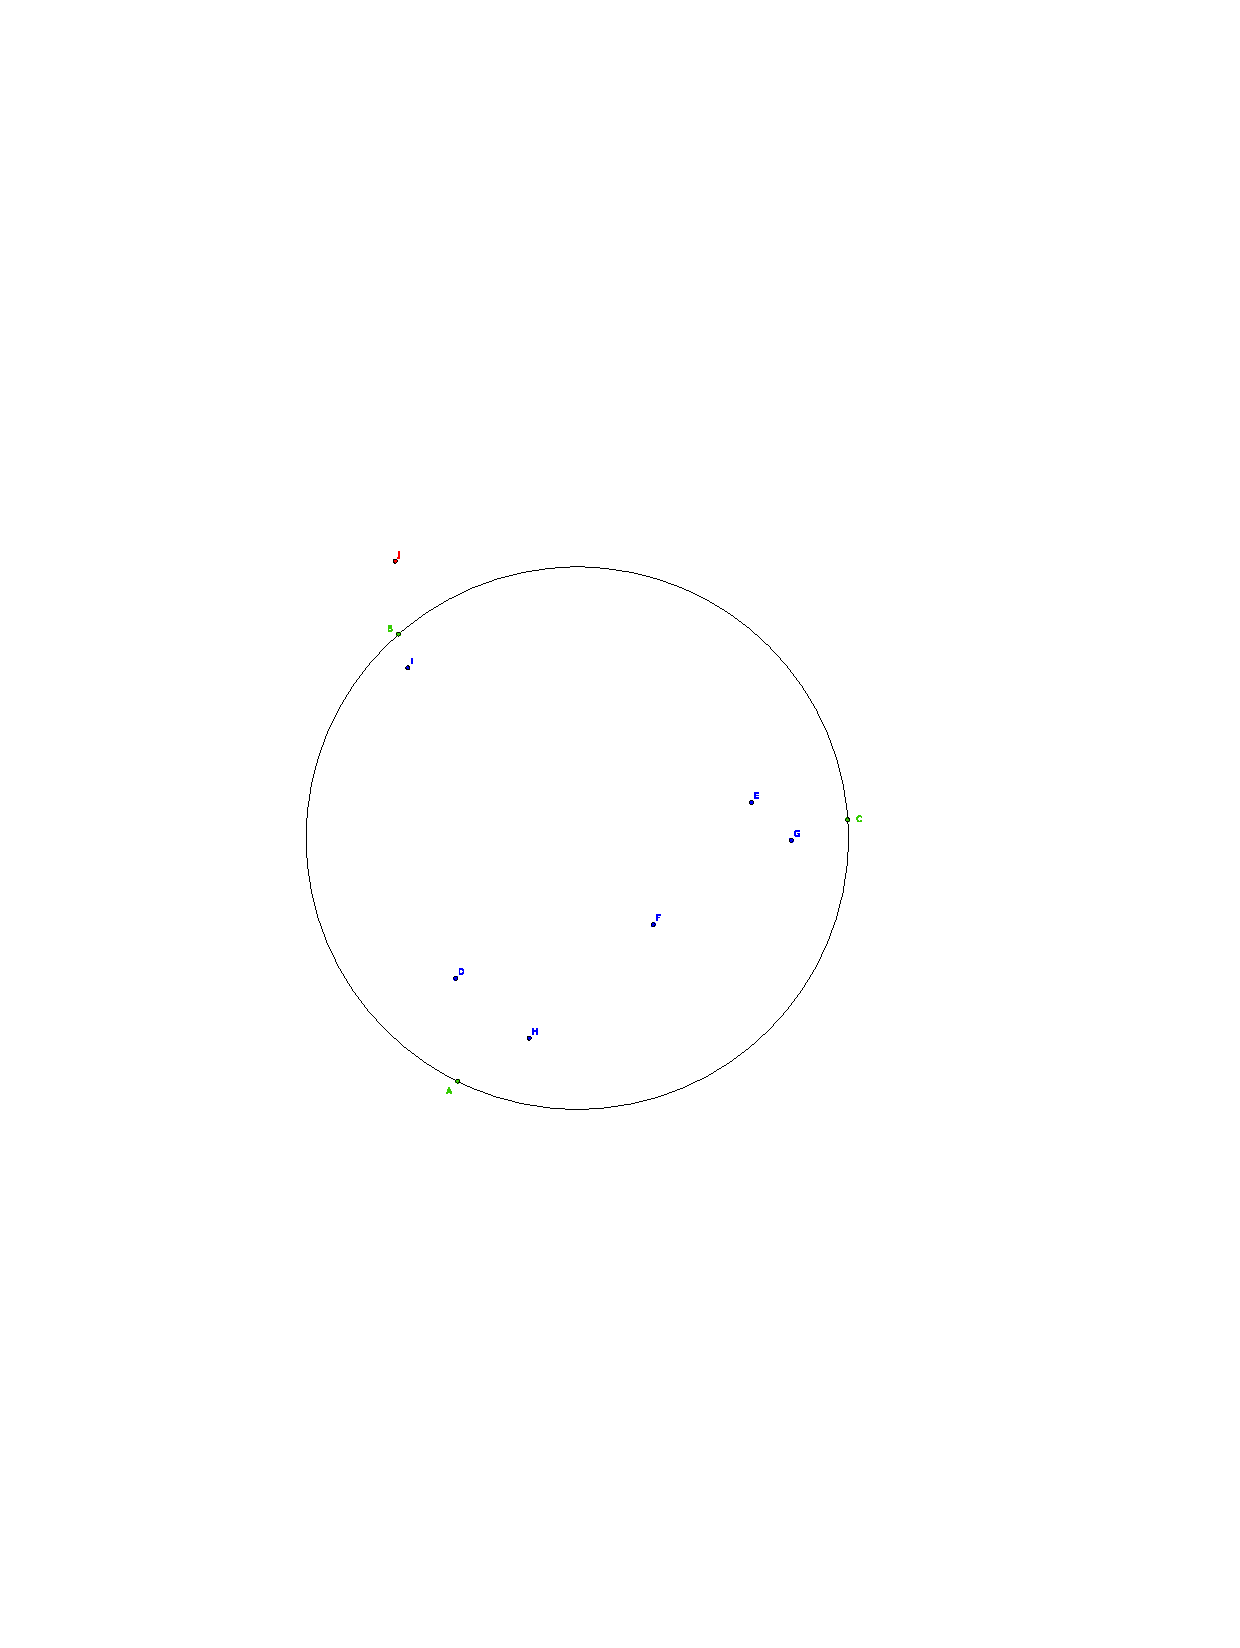
\includegraphics[trim=4cm 7cm 4cm 8.5cm, clip, width=0.7\textwidth]{figures/Next}
\end{frame}

\end{document}

